\documentclass[9pt]{scrreprt}
\usepackage{graphicx} % Required for inserting images
\usepackage[top=2.5cm, bottom=2.5cm, left = 1.5cm, right = 1.5cm]{geometry}
\geometry{a4paper}
\usepackage[utf8]{inputenc}
\usepackage{amsmath,amssymb}
\usepackage[pdftex,bookmarks,colorlinks,breaklinks]{hyperref}
\hypersetup{linkcolor=blue,citecolor=red,filecolor=black,urlcolor=black}
%\setlength{\headheight}{12pt}
\usepackage{times,subcaption,pdfpages}
\usepackage{listings}
\usepackage{float}
\linespread{1}
%\setlength{\parskip}{0.5em}
\usepackage{booktabs}
\usepackage[style=nature,backend=biber]{biblatex}
\usepackage{sectsty}
\chapterfont{\centering}
\sectionfont{\centering}

\begin{document}


\begin{titlepage}
   \begin{center}
       \large
       \vspace*{1cm}

       \textbf{ME5627 Measurements in Thermofluids }

       \vspace{0.5cm}
       
       \textbf{Laboratory Record}
       
       \vspace{6cm}

       \textbf{Submitted By\\~\\}
       {Rakesh S S 132414011 \\Vimal S V 132404001}


       \vspace{4cm}
     
       {
\includegraphics[width=4.5cm]{logos/iitpkd_fulllogo_color.pdf} \\}
       
       \vspace{2cm}   
       
       Department Mechanical Engineering\\
       Indian Institute of Technology Palakkad

       %\today           
   \end{center}
\end{titlepage}
\newpage

\chapter*{\normalsize EXPERIMENT 1}
\setcounter{chapter}{1}
\section*{\normalsize PART A: FAMILIARISATION WITH PC SCOPE AND BREAD BOARD THROUGH
RC CIRCUIT}
\textbf{Aim} – To gain familiarity with Bread Board, oscilloscope and oscilloscope data logger through RC circuit\\
\\
\textbf{Apparatus} – Bread board, wires, Oscilloscope, Resistor, capacitor\\
\\
\textbf{Details of Bread Board:}

\begin{figure}[H]
    \centering
    \begin{subfigure}[b]{0.57\textwidth}
        \centering
        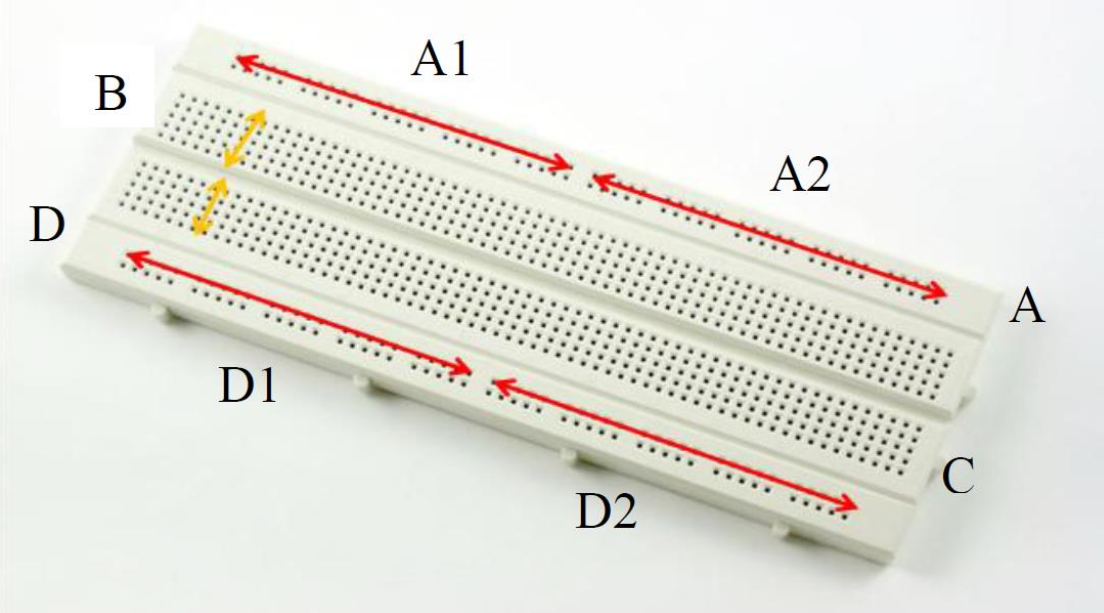
\includegraphics[width=\linewidth]{logos/Breadboard.png}
        \caption{Schematic of the Bread Board}
        \label{fig:Breadboard}
    \end{subfigure}
    \\
    \begin{subfigure}[b]{0.43\textwidth}
        \centering
        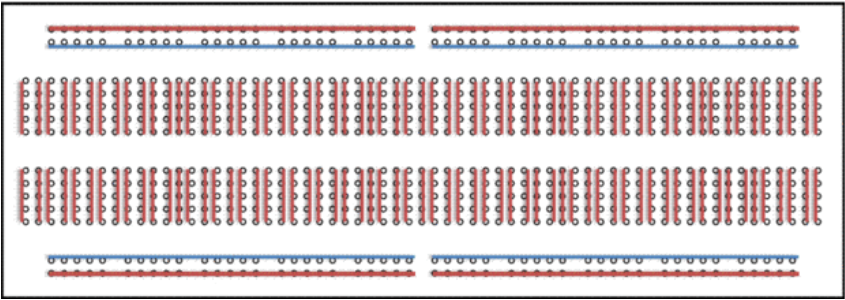
\includegraphics[width=\textwidth]{logos/Breadboard_connections.png}
        \caption{Equipotential lines}
        \label{fig:Breadboard_connections}
    \end{subfigure}
    \caption{Breadboard familiarisation}
    \label{fig:Breadboard familiarisation}
\end{figure}

\begin{itemize}
\item Hold the breadboard such that the horizontal side is longer than the vertical side.
\item There are four independent portions (A, B, C and D) created by three notches as in Fig.~\ref{fig:Breadboard}. Here, independence means portions A, B, C and D are not connected with each other
\end{itemize}

\textbf{\textit{Portion A and D}}
\begin{itemize}
\item Each portion of A and D is further subdivided into two regions as A1 and A2 shown in Fig.~\ref{fig:Breadboard familiarisation}.
\item Each horizontal line (shown through arrows in the Fig.~\ref{fig:Breadboard}) of A1, A2, D1 and D2 represent a single potential. Usually, as a general practice, these points are considered as ground for a given built circuit.
\end{itemize}

\textbf{\textit{Portion B and C}}
\begin{itemize}
\item In portion B and C, each vertical line (shown through arrows in Fig.~\ref{fig:Breadboard}) of B and C represents a single potential.
\item The above explanation can be better understood through Fig.~\ref{fig:Breadboard_connections} showing same potential lines.
\end{itemize}

\textbf{\textit{Details of oscilloscope probe}}\\

Fig.~\ref{fig:Oscilloscope_probe} shows a typical oscilloscope probe.

\begin{itemize}
\item The Oscilloscope probe is a passive connector which is used to connect oscilloscope to the electrical circuit. It consists of three parts Retractable hook tip (or crocodile clip), a Crocodile clip and BNC connector.
\item BNC connector: It is used to connect oscilloscope to the probe.
\item Retractable Hook tip: It is used to connect the node of the electrical circuit to the oscilloscope where there is a need to measure the signal.
\item Crocodile clip: It is connected to the ground of the electrical circuit in the bread board.
\item Make sure the RED slider on the probe should be on the X1 position only. X1 means amplification is unity.
\end{itemize}


\begin{figure}[H]
	\centering
	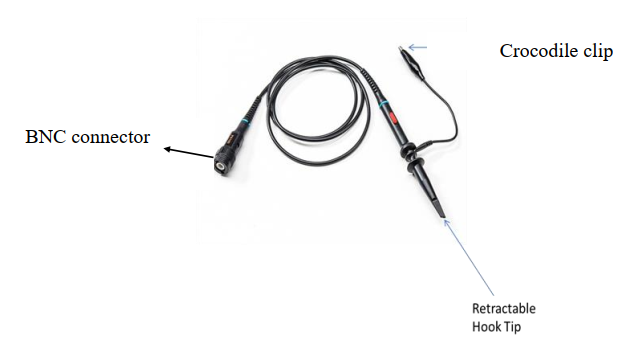
\includegraphics[width=0.6\linewidth]{logos/Oscilloscope_probe.png}
	\caption{PC scope probe}
	\label{fig:Oscilloscope_probe}
\end{figure}

\begin{figure}[H]
	\centering
	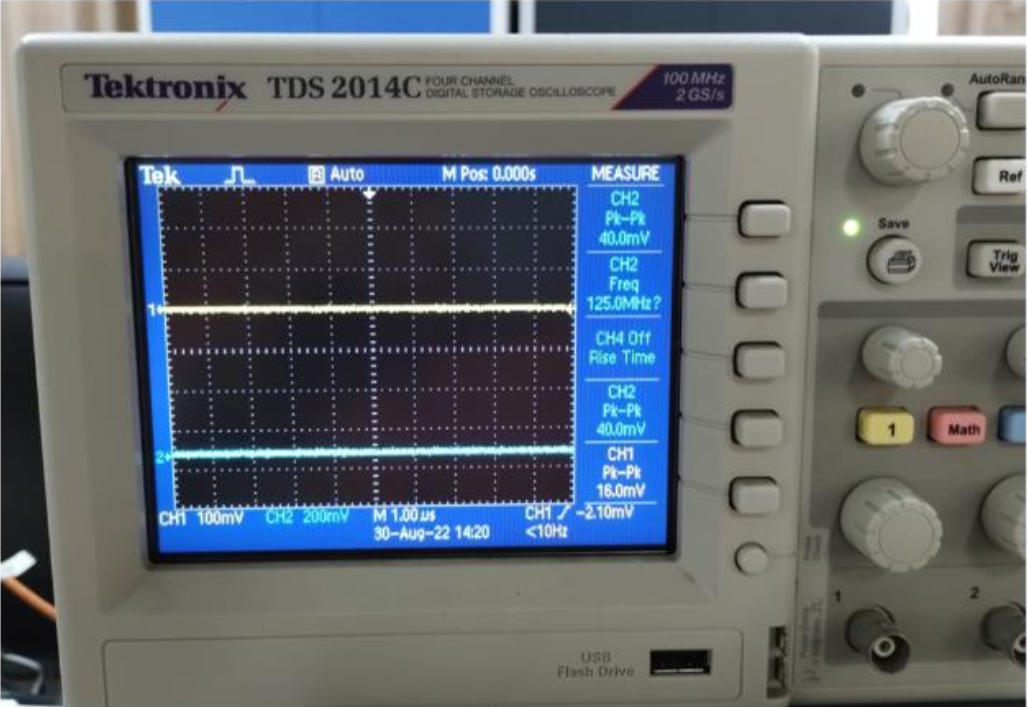
\includegraphics[width=0.6\linewidth]{logos/Oscilloscope.png}
	\caption{Four channel Oscilloscope with digital storage}
	\label{fig:Oscilloscope}
\end{figure}


Fig.~\ref{fig:Oscilloscope} shows a four channel Oscilloscope with digital data storage system. There are four
channels which displays the input/output signal. Input and output probes may be connected to any of these
four channels to visualize and analyze the waveforms of the signal. There are scaling, vertical and
horizontal controls to adjust the waveform in order to have better visualization. Peak to peak voltage and
time scale can be conveniently read from the monitor using the adjustment knob after pressing the cursor
button.

\begin{figure}[H]
	\centering
	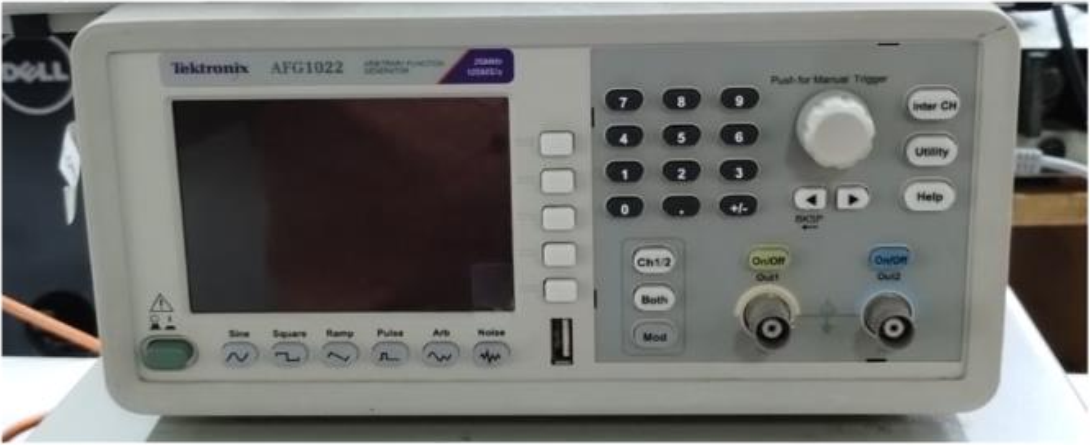
\includegraphics[width=0.7\linewidth]{logos/Function_Generator.png}
	\caption{Function Generator}
	\label{fig:Function_Generator}
\end{figure}

In order to obtain a desired input signal (sinusoidal, square, ramp, pulse or any arbitrary waveform) a function generator can be used (Fig.~\ref{fig:Function_Generator}). The desired amplitude and frequency of the waveform can be obtained using the side controls near the monitor. The output probes may be connected to any of the two channels. One of the crocodile clip of the output probe needs to be grounded and the other end can be given as input signal to generate the signal in the circuit. Also, in order to check whether the function generator is working, the probe may be connected to the Oscilloscope.\\
\\

\textbf{Calculation of Resistance:}
\begin{itemize}
\item Turn the resistor so that the gold or silver stripe is at the right end of the resistor.
\item Look at the color of the first two stripes on the left end. These correspond to the first two digits
of the resistor value. Use the table given below to determine the first two digits.
\item Look at the third stripe from the left. This corresponds to a multiplication value. Find the value
using the table below.
\item Multiply the two digit number from step two by the number obtained from step three. This is the
value of the resistor in ohms. The fourth stripe indicates the accuracy of the resistor.
\end{itemize}

\begin{figure}[H]
	\centering
	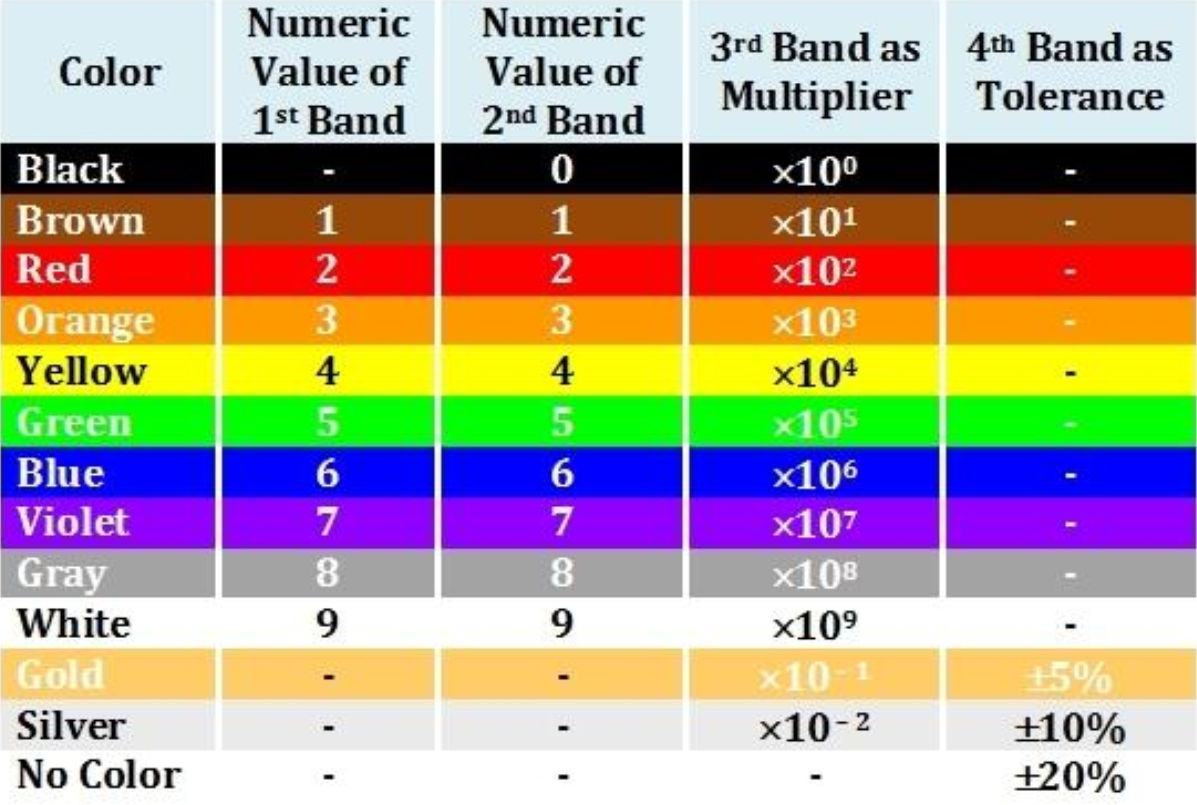
\includegraphics[width=0.7\linewidth]{logos/Resistance_colorcode.png}
	\caption{Resistance color code chart}
	\label{fig:Resistance_colorcode}
\end{figure}

\textbf{Sample:}


You are given a resistor whose stripes are colored from left to right as brown, black, orange, gold. Find
the resistance value.
\begin{itemize}
\item The gold stripe is on the right so go to Step Two.
\item The first stripe is brown which has a value of 1. The second stripe is black which has a value of 0.
Therefore the first two digits of the resistance value are 10.
\item The third stripe is orange which means x 1,000.
\item The value of the resistance is found as 10 x 1000 = 10,000 ohms i.e., 10~k$\Omega$ 
\item The gold stripe means the actual value of the resistor may vary by $5\%$ meaning the actual value
will be somewhere between 9,500 ohms and 10,500 ohms. (Since $5\%$ of 10,000 = 0.05 x 10,000 = 500)
\end{itemize}

\textbf{Calculation of Capacitance:}

\textbf{Sample Calculation:}
\begin{itemize}
\item Step 1: In the Fig.~\ref{fig:Ceramic capacitor}, the first two digits from the left indicates the first two digits of the
capacitor value. Here, in this case the first two digits are 1 and 0. Therefore, the first two digits of
the capacitor value is 10.
\item Step 2: The third digit is 4 which means that four zeroes would be followed by 1 (10,000 pF).
\item The value of the capacitor is found out to be the product of the number obtained in step 1 and step
2. That is, 10 $\times$ 10000 = 10,0000 pF i.e 0.1 $\mu$F.
\end{itemize}

\begin{figure}[H]
	\centering
	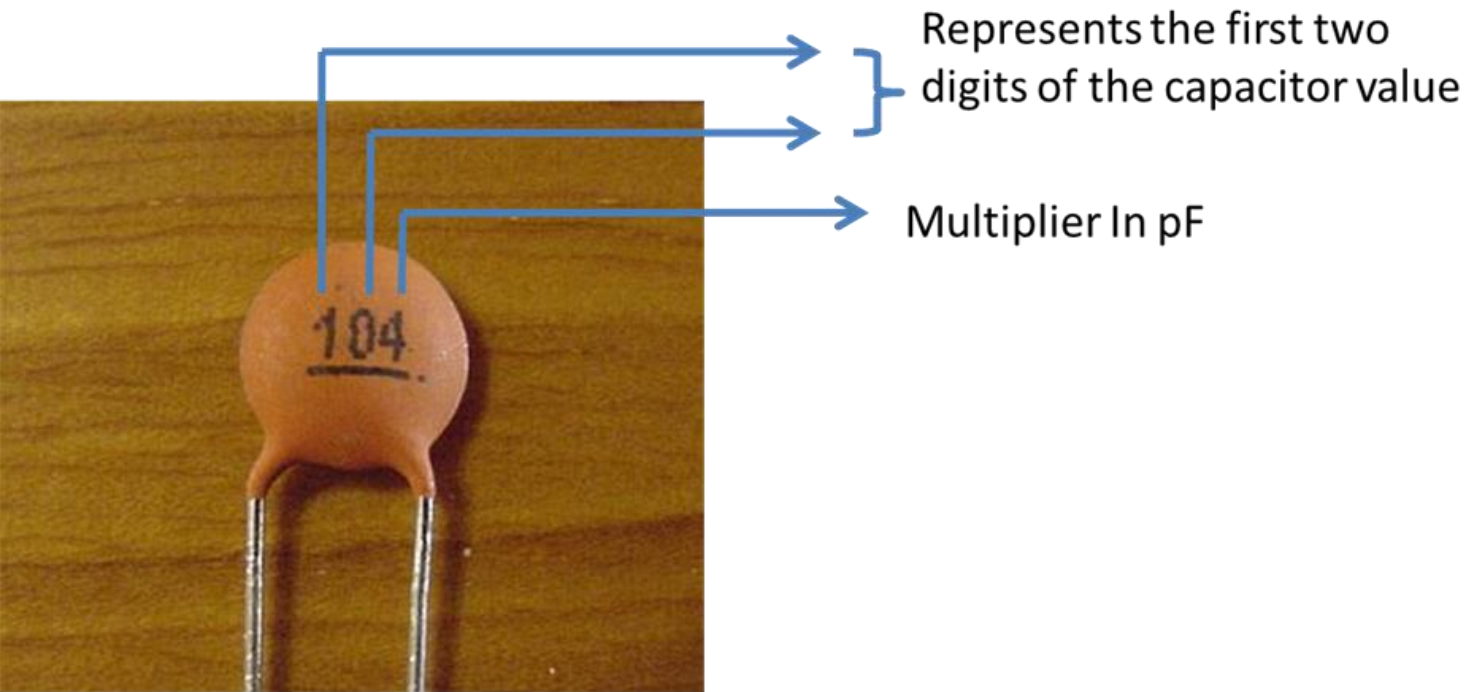
\includegraphics[width=0.8\linewidth]{logos/Ceramic_capacitor.PNG}
	\caption{Ceramic capacitor}
	\label{fig:Ceramic capacitor}
\end{figure}

\textbf{Circuit Diagram:}\\
\par Figures.~\ref{fig:RC circuit} and~\ref{fig:PC scope} show the RC circuit and PC scope
\begin{figure}[H]
\centering
\begin{minipage}{.5\textwidth}
  \centering
  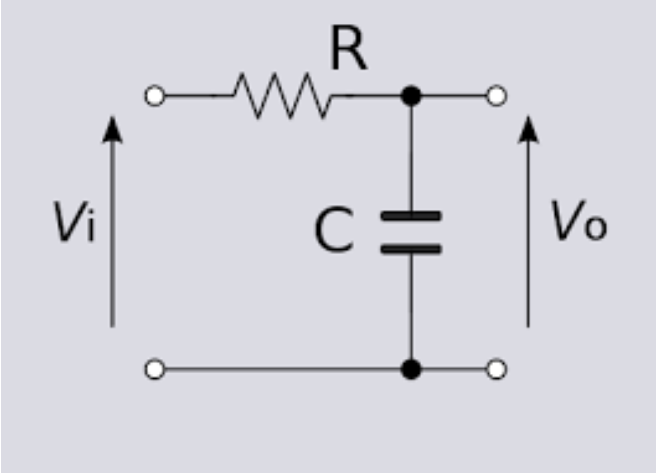
\includegraphics[width=6cm]{logos/RC_circuit.png}
  \caption{Typical RC circuit.}
  \label{fig:RC circuit}
\end{minipage}%
\begin{minipage}{.5\textwidth}
  \centering
  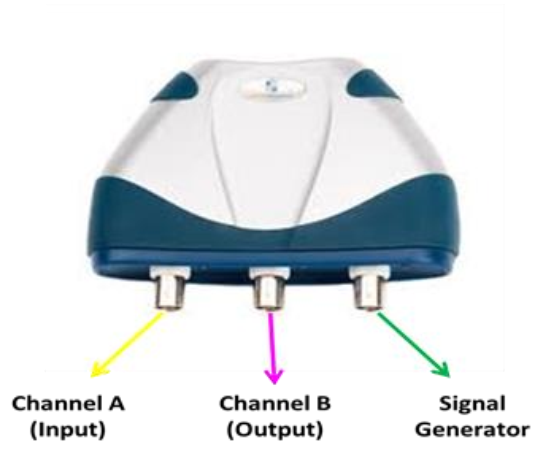
\includegraphics[width=5cm]{logos/PC_scope.png}
  \caption{PC Scope.}
  \label{fig:PC scope}
\end{minipage}
\end{figure}


\textbf{Experimental Procedure:}
\begin{itemize}
\item Build an RC circuit as shown in the Fig.~\ref{fig:RC circuit} on the bread board.
\item \textit{\textbf{Circuit input to the oscilloscope}}\\
First PC scope probe is taken. BNC connector of this oscilloscope is connected to the input of the oscilloscope shown in Fig.~\ref{fig:PC scope}. Connect the retractable hook tip of the oscilloscope probe (inputprobe) to the open end of the resistor. The crocodile clip of this input PC scope probe is connected to the ground of the bread board.
\item \textit{\textbf{Circuit Output to the oscilloscope}}\\
Second oscilloscope probe is taken. BNC connector of this oscilloscope is connected to the output of the scope shown in Fig.~\ref{fig:PC scope}. Connect the retractable hook tip of the scope probe (output probe) to common junction of resistor and capacitor. The crocodile clip of this input oscilloscope probe is connected to the ground of the bread board.
\item \textit{\textbf{Desired Signal Input to the oscilloscope}}\\
Third oscilloscope probe is taken. BNC connector of this oscilloscope is connected to the signal generator of the oscilloscope shown in Fig.~\ref{fig:PC scope}. Connect the retractable hook tip of the oscilloscope probe (input probe) to the open end of the resistor. The crocodile clip of this input oscilloscope probe is connected to the ground of the bread board.
\end{itemize}

Following flow chart shows the flow of input and ouput signals.

\begin{figure}[H]
	\centering
	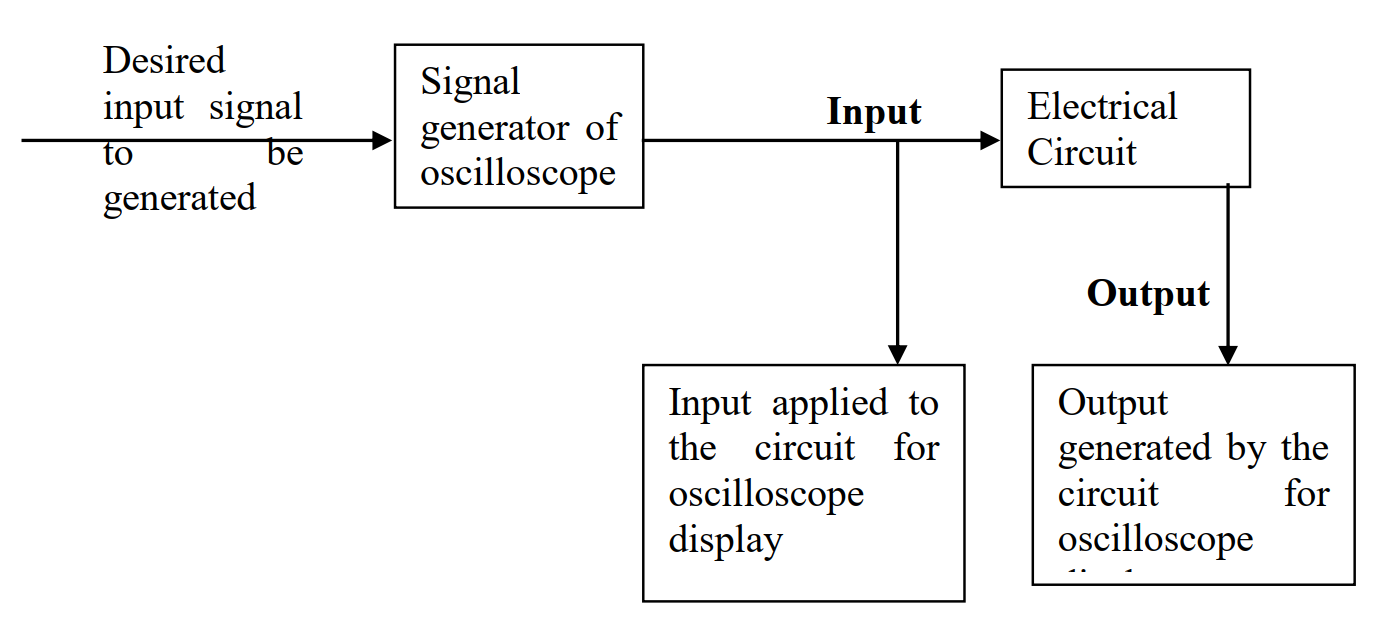
\includegraphics[width=0.8\linewidth]{logos/Flow_chart_IO.PNG}
	\caption{Flowchart indicating the flow of input and output signals}
	\label{fig:Flow chart IO}
\end{figure}

\begin{itemize}
\item There is switch on the probe. Make sure that switch is towards ‘X1’ side so that the values are not amplified by the probe.
\item Give sinusoidal signal of very low amplitude (2 V) as input and observe the output.
\item Increase the amplitude of the input signal and observe the output, repeat this step three times.
\item Measure the peak voltage of both input and output signal using meter A and B.
\item Try giving some other type of signal at some other frequency and observe/measure the output.
\end{itemize}

\textbf{Conclusions/Discussions on the results:}
\newpage
\section*{\centering EXPERIMENT 1}
\section*{\normalsize PART B: BASIC WORKING OF INSTRUMENTATION OP AMP (INA 129)}
\textbf{Aim} – To study the basic working of Instrumentation op amp (INA129)\\
\\
\textbf{Apparatus} – INA 129, Bread board, wires, dc power supply, Oscilloscope\\
\begin{figure}[H]
	\centering
	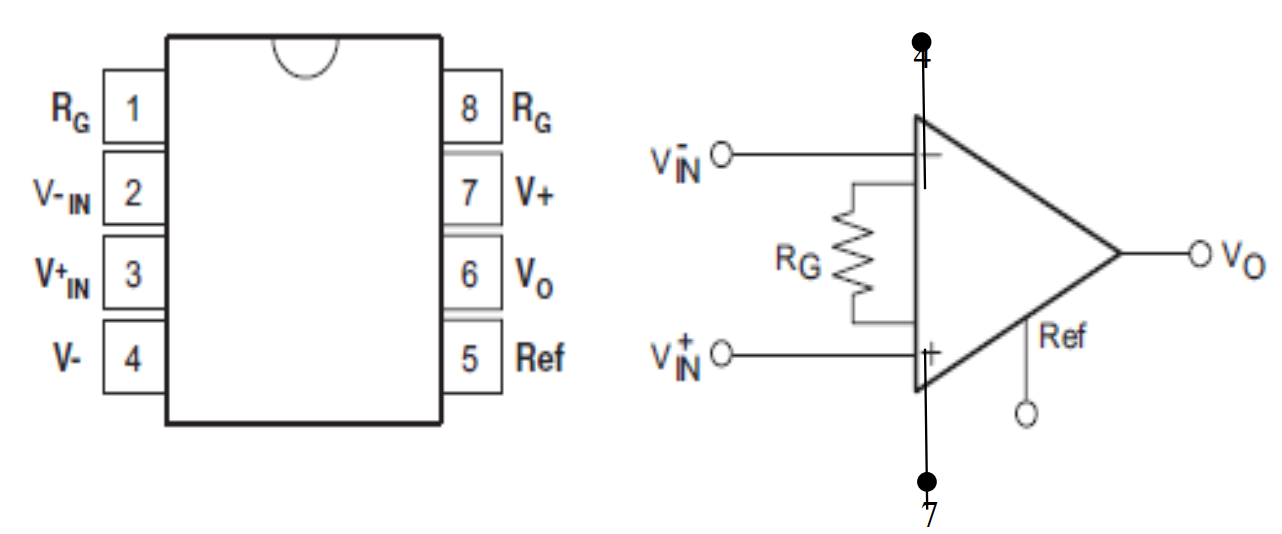
\includegraphics[width=0.8\linewidth]{logos/OP-Amp.PNG}
	\caption{Schematic of the instrumentation operational amplifier with pins (INA 129)}
	\label{fig:OP-Amp}
\end{figure}

\textbf{Experimental Procedure}

\begin{itemize}
\item Make the circuit as shown in the Fig. 1.8 on the bread board.
\item Connect the Retractable hook tip of the input probe and signal generator probe of the oscilloscope at pin 3 and the crocodile clip of both the probe (input and signal generator) at pin 2 of INA 129.
\item Connect the Retractable hook tip of the output probe at pin 6 and the crocodile clip of the output probe at pin 5 of INA 129. Make a virtual ground in the breadboard and connect pin 5 to this virtual ground.
\item Select the value of RG based on desired gain. The relation between $R_G$ and gain/Amplification (G) is given in Table.~ref{tab:Rc and gain}
\item Connect the resistance RG across pin 1 and 8 of INA 129.
\item D.C power supply is set to 12V whose positive end is connected to pin 7 while its negative end is connected to pin 4.
\item Give sinusoidal signal of 200mV amplitude and the frequency of 300 Hz in the signal generator and observe the output at the interface of oscilloscope in the monitor. Ensure that pin 5 is grounded.
\item Change the value of $R_G$, repeat the above procedure and observe the output.
\item Note down the output in the observation Table.
\end{itemize}

\end{document}